\documentclass[output=paper]{langsci/langscibook} 
\author{Wendy Fox\affiliation{Johannes Gutenberg University of Mainz/Germersheim}}
\title{Integrated titles: {A}n improved viewing experience?}
\abstract{While there are a few examples of (sub)titles placed individually in the image as a means of translation of an additional language into the film’s main language, this practise has not yet been used to commercially translate a complete film for a foreign target audience. Using eye tracking data, this study examines to what extent the placement and design of (sub)titles affect reading time and the visual perception of the image. The applied placement strategies were based on the undistracted focus points of 14 English native participants and image composition principles from film studies. Additional 31 German participants with little or no knowledge of English watched the English film with traditional subtitles or integrated titles. The results of the eye tracking data analysis indicate that, while reaction time (time to first fixation) increases, the reading time (total visit duration) for integrated titles decreases, the viewers are less likely to focus on the title area before the title appears and their focus resembles the undistracted gaze behaviour of the native participants to a much greater degree. Additionally, the split attention between image and title shifts towards the image. Integrated titles appear to motivate the viewer to return to the focal points faster and spend more time exploring the image in between titles. Their placement allows for shorter saccades and thereby decreases the time in which no visual information is obtained.}

% \chapterDOI{}
\maketitle
\begin{document}



\section{Introduction}

Historically a dubbing country\footnote{For the history of dubbing in Germany, refer to http://www.sprechersprecher.de/blog/die-geschichte-der-film-synchronisation-in-deutschland [30.12.2014, in German].}, 
Germany is not well-known for subtitled productions. However, while dubbing is obviously predominant in Germany and other neighbouring countries with a similar language-related history and a sufficiently large target audience, more and more German viewers prefer the original versions of English film productions.\footnote{This is reflected in the increasing number of screenings of original versions in German cinemas (see for example http://www.koeln.de/kino/ov-filme [16.12.2014, in German] and http://against-dubbing.com/de/ovkinos/ [16.12.2014, in German]), especially since the introduction of digital film, changing from 35mm film to digital projection. This allowed for a considerably easier and more cost-efficient process for film distributors (see http://www.dw.de/der-35mm-film-stirbt-aus-kino-wird-digital/a-17013764 [16.12.2014, in German]). 
} 
Fans of series such as \textit{Game of Thrones} (HBO, USA/UK 2011-) or \textit{The Big Bang Theory} (CBS, USA 2007-) yearn for every new episode and many do not want to wait for the German dubbed version. Combined with the desire for a more authentic film experience, many German viewers prefer original and subtitled versions of their favourite show.\footnote{This assumption is supported by the increasing number of German internet forums that centre around creating and providing fansubs – subtitles created by fans – for download: subcentral.de with approximately 134 new posts per day, subtitles.de, tv4user.de and opensubtitles.org [30.12.2014].
}


Traditional subtitling can be seen as a strong intrusion into the original image composition that may disrupt or even destroy the director’s intended shot composition and focal points. But isn’t the carefully composed interplay of image and sound what makes film “the most popular art form” \citep[p. 35]{mercado2010} of today’s entertainment landscape? Long saccades between focal points and subtitles affect the viewer’s information intake and in particular the German audience, who are not used to subtitles, seems to prefer to wait for the next subtitle instead of looking back up again.\footnote{This is indicated by the high amount of fixations in the subtitle area before the subtitle actually appears, as explained in Figure \ref{fox:fig:8} in chapter 4.1.} Furthermore, not only the placement, but also the overall design of traditional subtitles can disturb the image composition – for instance titles with a weak contrast, inappropriate typeface or irritating colour system. So should it not, despite the translation process, be possible to preserve both image and sound as far as possible by designing and placing subtitles differently? Today’s numerous artistic and technical possibilities combined with the immense amount of work that goes into the visual aspects of a film, taking into account not only special effects, but also typefaces, opening credits and text-image compositions, should enable producers to do so. A further development of existing subtitling guidelines would not only express respect towards the original film version but also the translator’s work.


The present study is based on Just and Carpenter’s strong eye-mind hypothesis, which states that “there is no appreciable lag between what is fixated and what is processed” (1980,~331). Caffrey notes a recent increase in “output from researchers into the perception of translated AV content employing data generated with eye trackers” (2009,~4), mentioning Moran (2008) and Del Missier (2008). Cognitive psychologists such as d’Ydawelle et al. (1985), Koolstra et al. (1999) and d’Ydawelle/de Bruycker (2007) analysed fixation-based eye tracking data such as the perception of one- and two-liners, while \citet{kruger2013} discuss the impact of subtitles on the cognitive load and support their hypotheses with eye tracking data. Most research on new forms of subtitles relates to fan-produced subtitles (Nornes 1999, Ferrer Simó 2005, Pérez Gonzáles 2007, Díaz Cintas/Muñoz Sánchez 2006, Orrego Carmona 2014) and only a few focus on commercially oriented subtitles (Díaz Cintas 2005, Caffrey 2009). \citet{caffrey2009} and \citet{mcclarty2012, mcclarty2013a, mcclarty2013b} present two of the more recent eye tracking-based studies on innovative subtitling methods. There are already several terms that attempt to grasp these new subtitling concepts and designs: “abusive subtitles” (Nornes 1999, 2004) describes the experimental use of subtitles in regard to both graphical and linguistic aspects while the terms “hybrid” \citep{cintas2006} and “creative” \citep{mcclarty2012} subtitles focus on the overall presentation and are presented in opposition to traditionally placed and designed subtitles. Even though these terms cover many of the differences between traditional subtitles and more recent concepts, they do not seem to apply to the titles used in \citet{fox2012} and the present study as they might still refer to subtitles being automatically placed in the bottom (or top) area of the screen. Therefore, the term “integrated titles” \citep{fox2012} was used, referring to titles being integrated\footnote{Inspired by Bayram/Bayraktar who described “text information [that is placed] directly into the picture” (2012,~82) as “integrated formats” (ibid.).\par 
} into the shot composition. At the same time, this term describes the novelty of the present study: So far, there have been no eye tracking studies of German integrated titles\footnote{For studies on integrated titles in English, see Mc\citet{mcclarty2013b} and \citet{brown2015}.\par 
} or –  as Germany is traditionally a dubbing country – much research on subtitling in general. Additionally, no eye tracking study has been conducted on the aesthetics and perception of subtitles combined with attempts to draft a new, updated set of guidelines for recent subtitling concepts.


While there are only a few examples of English productions that use individually placed titles – for instance \textit{Man on Fire} (Twentieth Century Fox, USA/UK 2004), \textit{Heroes} (NBC, USA 2006-2010) and \textit{Slumdog Millionaire} (Warner Bros., USA/UK 2008) – there are even fewer examples of recreations of these kinds of “text inserts” \citep{molerov2013} and titles for the German version, e.g. the series \textit{Sherlock} (BBC/Hartswood Films 2010-) and \textit{Stark Trek Into Darkness} (Paramount Pictures, USA 2013). Creatively placed titles such as in \textit{Heroes} and \textit{Man on Fire} were removed during the translation process into German and traditional subtitles accompanied the dubbed version.



This research is relevant not only because of the increasing use of integrated titles in English film productions but also because of the fact that “even though these translation and accessibility services only account for 0.1\% – 1\% of the budget of an average film production (Lambourne 2012), over half of the revenue of, for example, both top-grossing and award-winning Hollywood films comes from foreign territories” \citep[p. 202]{romero2013}. Therefore, it is only in the interest of film producers to take a critical look at the perception of the translated version of their film and studies on more content- and image-related ways of audiovisual translation might be helpful in motivating this shift. An alternative placement of titles might allow for a positive split attention towards the image and therefore enable a viewing behaviour more similar to that of the native audience and closer to the intended focal points, while taking into consideration both image composition and typographic identity of the film.




A previous pilot study \citep{fox2012} examining the first episode of the British TV series \textit{Being Human} (BBC/Touchpaper, UK 2008-; so far without official German subtitles or dubbing) evaluated whether integrated titles improve understanding without interfering with the composition and aesthetics of the episode. In a basic three-step-experiment, the advantages and disadvantages of integrated titles were analysed by recording the eye movements of 45 participants. The results indicated that the reduced time spent on (long) saccadic eye movements gives viewers more time to focus on the image and makes it easier for them to link the titles to the plot. Moreover, the film material was perceived as more aesthetic and closer to the original version.


The present eye tracking study addresses whether the individual placement and design of (sub)titles affect the viewer’s reading time, the time spent exploring the image (rather than waiting for the next title) as well as the overall viewing experience, including the time spent on the intended focal points and the split attention between image and (sub)title. Additional thought was given to indicating speech direction and rate as well as speaker position. While the study also included the creation and translation of the necessary subtitles and integrated titles, the present article focuses on the eye tracking experiment and its results. Pablo Romero-Fresco gave his permission to use his short documentary \textit{Joining the Dots} (UK 2012) and agreed to discuss his image system and shot compositions as a first step to creating the integrated titles. These were based on adjusted traditional guidelines, guidelines created during previous work \citep{fox2012} and a first sketch of the modular guidelines that are presented in \citet{fox2015}. 14~English native participants watched the film without subtitles in order to define the most common focus points\footnote{Note that, while the ‘focal points’ refer to the intended focus created by the director using image composition and technical elements, the ‘focus points’ are areas fixated by the majority of the participants.} and provide reference data. 15 native speakers of German with little or no knowledge of English\footnote{According to the participants’ own statements.\par 
} watched the film with traditional subtitles and an additional 16~German native-speakers with little or no knowledge of English\footnote{  According to the participants’ own statements.\par 
} watched the film with integrated titles. The gaze behaviour of the German participants was analysed in regard to reaction times (time to first fixation), reading times (total visit duration) and general visual attention distribution between image and (sub)title.

Based on the pilot study \citep{fox2012}, expected results are decreased reading times and a gaze behaviour more similar to that of the English native speakers. It is to be assumed that the reaction time for integrated titles is slightly longer than for traditional titles. Due to the individual placement of the titles, the distance between focal point and title is on average smaller and the viewer would therefore gain more time to explore the image and focus on the focal points. Overall, expectations are that integrated titles will have a positive effect on both the aesthetic viewing experience of the audience and the split-attention between image and title, as integrated titles appear to motivate the viewer to return to the main focal point faster and spend more time exploring the image in between titles.

\section{Materials}

Of the 45 participants, 14 were native speakers of English between the age of 18 and 45 who study at the FTSK\footnote{Abbreviation for “Fachbereich Translations-, Sprach- und Kulturwissenschaft“, the “Faculty of Translation Studies, Linguistics and Cultural Studies” in Germersheim and part of the Johannes Gutenberg University of Mainz.} and watched the original version of \textit{Joining the Dots}. As film audiences are usually not homogenous groups, no other characteristics besides native language and eye sight were determined. Each participant claimed to have normal or corrected-to-normal vision. Thirty-one participants were German native speakers who stated that they rely on German subtitles to understand English films. As using subtitles is a personal decision based on the viewer’s self-assessment and not his or her factual knowledge of the foreign language (and on availability), the actual level of the participants’ English was not determined. Of these participants with German as their native language, 15 randomly chosen participants watched \textit{Joining the Dots} with traditional subtitles in German. The other 16 German participants watched the film with the integrated titles. None of the participants had seen the film before.


\textit{Joining the Dots} is a short documentary by Pablo Romero-Fresco, screened for the first time in 2012.\footnote{For further information on Joining the Dots, see http://www.jostrans.org/issue20/
int\_romero.php [28.10.2014]} The documentary shows an interview with Trevor Franklin who went blind at the age of 60. He speaks about his experiences and how he handles the disability. The main topic of the documentary is accessibility for the blind, focusing on television and theatre. In an interview with Pablo Romero-Fresco, the image system, compositions and key elements in the various scenes were defined and possible placements and designs discussed. Due to its documental character, \textit{Joining the Dots} offers a simple image system\footnote{For a definition of “image system” see Mercado (2010, 21): “[…] refers to the use of recurrent images and compositions in a film to add layers of meaning to a narrative. … Because the experience of watching a film relies so much on the use of images ([…]), most films have an image system at work at some level, whether the filmmaker intends to have one or not.” It is important to distinguish between the image system of a film and the individual “shot compositions” (ibid.) of a scene.} and clearly structured shot compositions. Frontal shots of the persons being interviewed are predominant (see \ref{fox:fig:1}) while further scenes introduce important places in Trevor’s life such as the theatre or his home. The interview situations and several other rather static scenes (see \ref{fox:fig:2}) are well suited for integrated titles as the primary and secondary areas are quite clear and the secondary area offers enough space for the titles. Due to their rather static character, there is no immense risk of important elements being covered by the titles.


\begin{figure}
 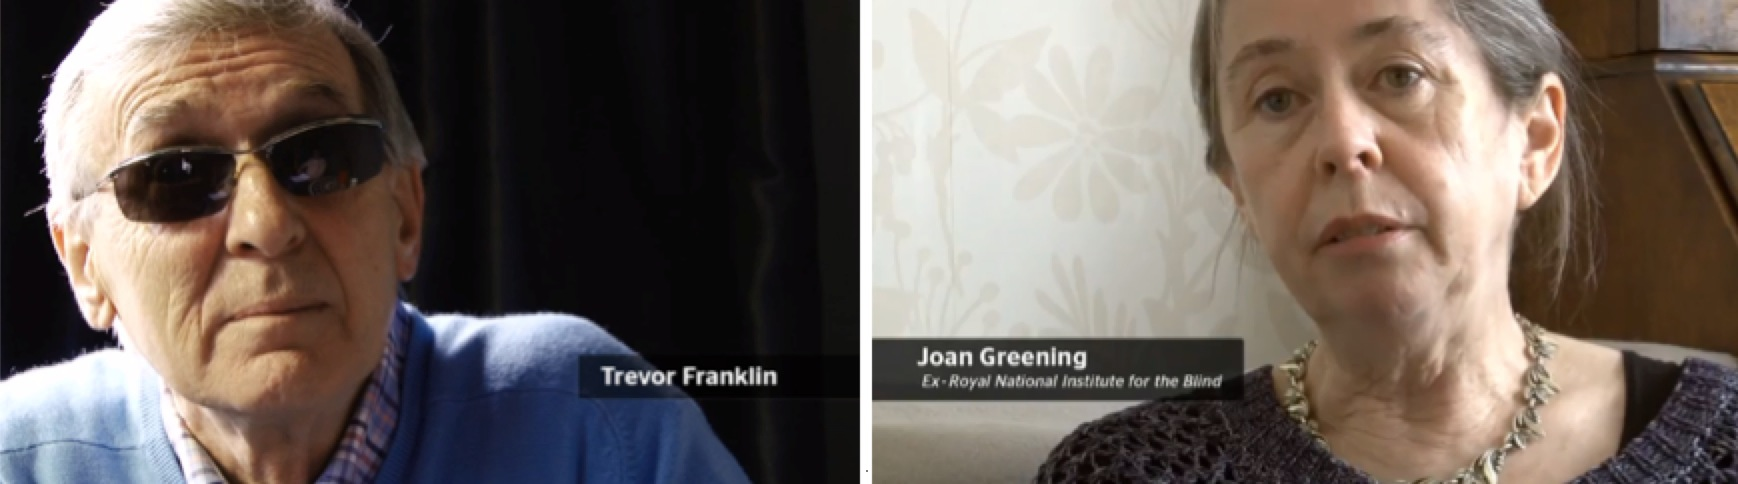
\includegraphics[width=\textwidth]{figures/Fox1.png}
 \caption{Frontal shots of the interviewees in Joining the Dots (UK 2012}
  \label{fox:fig:1}
\end{figure}  

\begin{figure}
 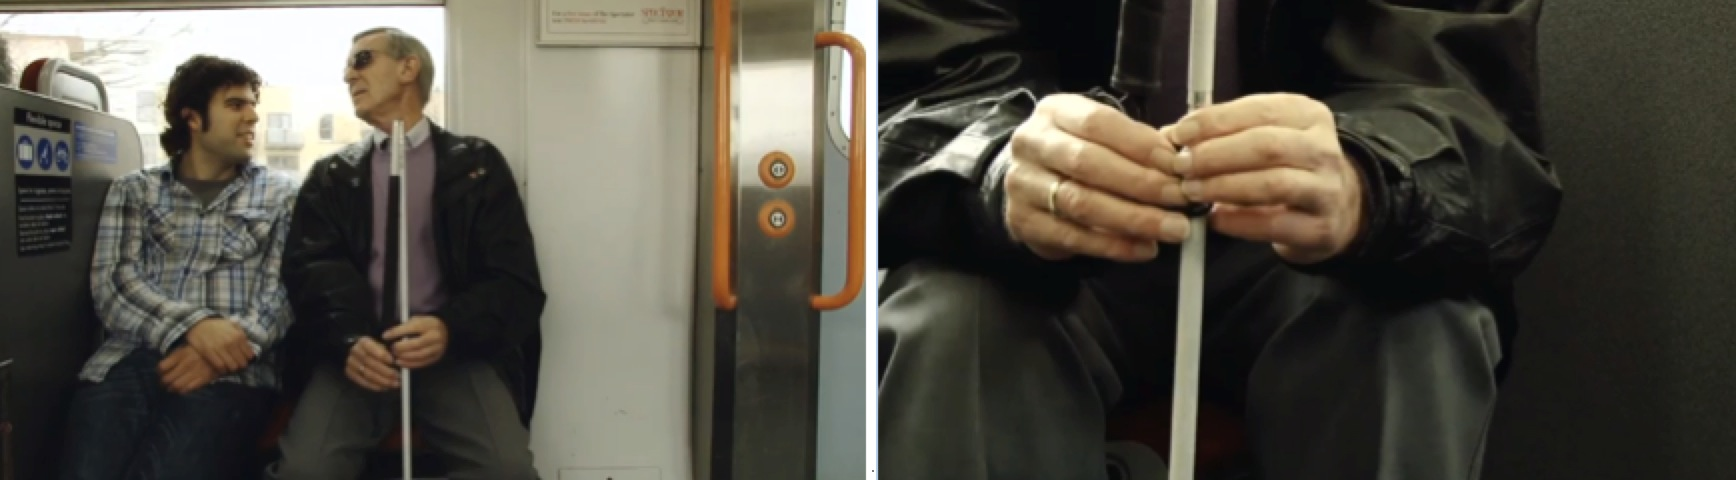
\includegraphics[width=\textwidth]{figures/Fox2.png}
 \caption{Static scenes with evenly balanced primary and secondary areas (Joining the Dots, UK 2012)}
 \label{fox:fig:2}
\end{figure} 



The definition of primary and secondary areas is based on the analysis of the image composition and the resulting focal points in the image. According to Mercado, “focal points refer to the center of interest in a composition, the area where the viewer’s gaze will gravitate to because of the arrangement of all the visual elements in the frame.” (2010,~11) Thus, the combination of several technical aspects such as the used lenses that define the sharp areas in the image automatically attracts the viewer’s gaze to where the director wants it to be. These are seen as primary areas and should not be covered by text. Other concepts that can help to define primary and secondary areas and “isolate the subject within the frame” (ibid. 2010,~35) are the “rule of thirds” (ibid. 2010,~7), “Hitchcock’s rule” (ibid.), “balanced/unbalanced compositions” and the overall “visual weight” (ibid. 2010,~8) of elements in the shot composition. The eye tracking recordings with the English native-speakers confirmed this theory and allowed for the distribution based on the eye tracking data. \ref{fox:fig:3} shows an example of a heat map of the focus points of the English native participants and the corresponding definition of the primary and secondary areas.


\begin{figure}
 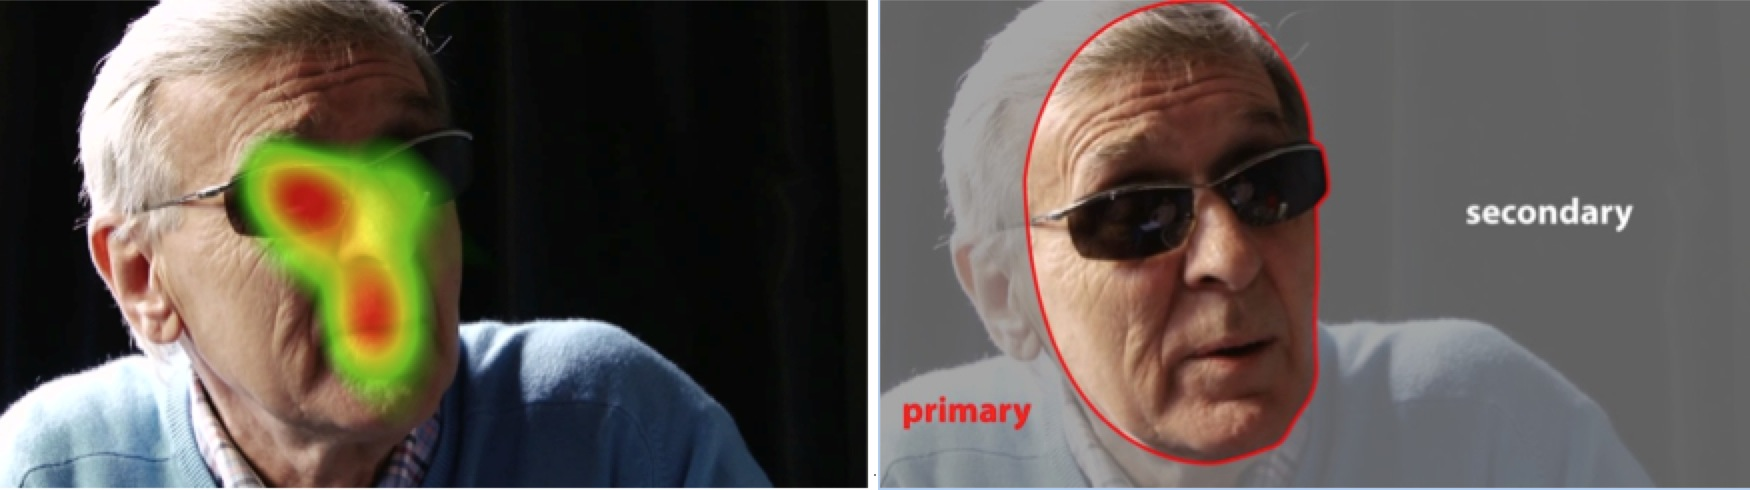
\includegraphics[width=\textwidth]{figures/Fox3.png}
 \caption{Fixation points of English natives (left) and resulting primary/secondary areas (Joining the Dots, UK 2012)}
 \label{fox:fig:3}
\end{figure}  



Aside from these rather static image compositions, \textit{Joining the Dots} includes several recurring compositions. Images with mainly blurred or fast moving elements underline the interviewee’s statements, for example as Trevor speaks about the progressing loss of his sight (see \ref{fox:fig:4}).


\begin{figure}
 
\includegraphics[width=\textwidth]{figures/Fox4.png}
 \caption{Scenes that support the overall atmosphere in Joining the Dots (UK 2012)}
 \label{fox:fig:4}
\end{figure} 



The German subtitles were created according to the traditional guidelines described by \citet{ivarsson1998} and \citet{karamitroglou1998}. The integrated titles consisted of the same translation but were modified according to the discussion of traditional guidelines in \citet{fox2012}. These modifications included more individual fade durations and a much scarcer use of the three dots at the end of a title. For aesthetical reasons, no commas were placed at the end of a title and dialogs were not combined in the same title for the sake of improved speaker identification. No italics were used to indicate a speaker outside the shot as it is very clear throughout the whole documentation whether the speaker is visible in the current shot or not. Even though this version of \textit{Joining the Dots }is intended for a hearing audience and the modifications are based on the assumption that the audience can connect the visible with the audible content, adjustments such as the individual placement might already provide additional information for the hearing-impaired. For a more accessible translation, useful visual elements need to be re-evaluated and adjusted to the needs of the respective target group.


\subsection{Placement }

As the interviews are the main element of the documentary, it was decided not to place every title individually but rather define rough areas of title placement for the three interviewees. Therefore, Trevor’s titles are displayed in the right half of the image as he tends to look to the right. The titles for Joan Greening and Mags Silbery are displayed on the left half as they tend to look to the left. These positions were also supported by the positions of the captions with their names (see \ref{fox:fig:1}) and the secondary areas in the corresponding shot compositions. \ref{fox:fig:5} illustrates how the secondary areas often allow for a more even and stronger contrast. Keeping the positions of the placements to a minimum, even if the shot composition changes noticeably, might allow for more accessible adjustment, for instance for a hearing-impaired or deaf audience. For such an audience, with a possibly greater need for additional visual information, speaker-related positions allow for faster identification of the speaker, even if he or she is not visible on the screen. Colour is another possibility to make identification easier, even though it is not always easy to come up with a suitable colour concept for a film that works throughout the whole story.

\begin{figure}
 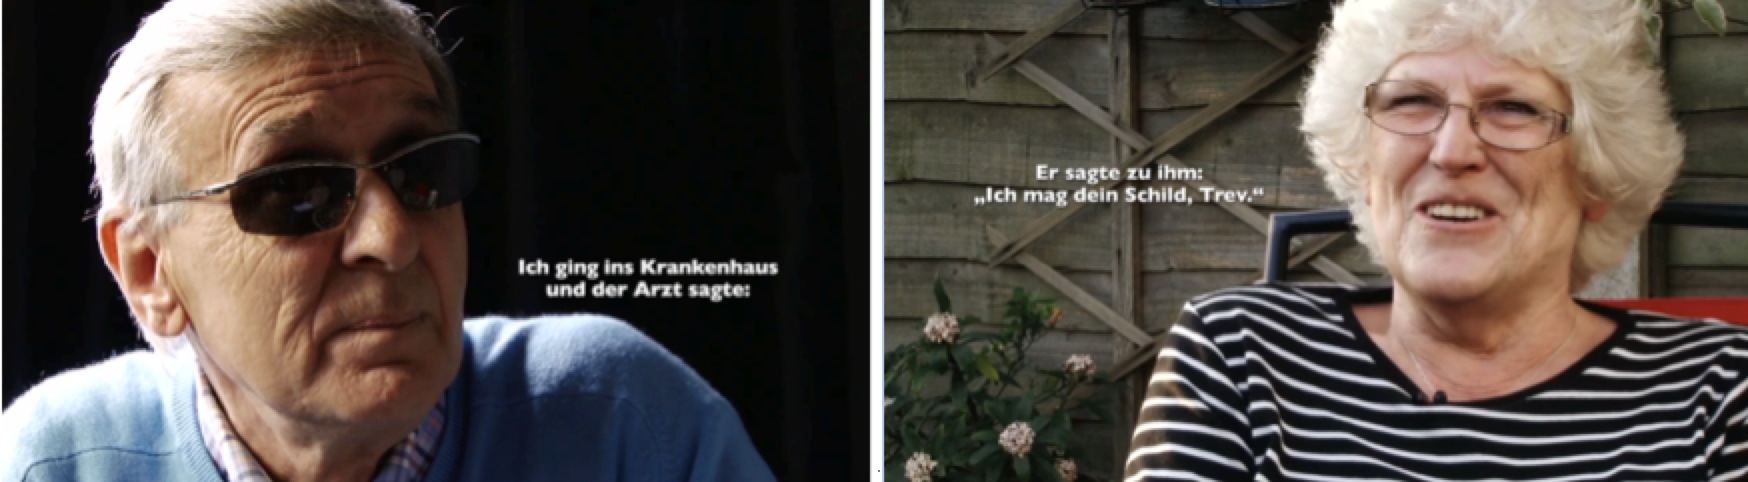
\includegraphics[width=\textwidth]{figures/Fox5.png}
 \caption{Roughly defined areas for Trevor (to the right of the speaker) and Mags (to the left of the speaker)(Joining the Dots, UK 2012)}
 \label{fox:fig:5}
\end{figure} 


\subsection{Typography}

The original version of \textit{Joining the Dots} used two typefaces: Today’s MS Office standard typeface \textit{Calibri}\footnote{For further information on the typeface \textit{Calibri}, see http://www.lucasfonts.com/case-studies/calibri-consolas/ [29.12.2014]} to display names (see \ref{fox:fig:1}) and \textit{Slab Serif}\footnote{For further information on the typeface \textit{Slab Serif}, see http://www.linotype.com/3493/ introduction.html [29.12.2014\}} for the film title. The closing credits are a mixture of both typefaces. The title design for \textit{Joining the Dots} was based on a detailed interview with the director Pablo Romero-Fresco and the analysis of the existing examples of integrated titles and creative solutions. After various typographic tests with typefaces and spatial effects, the typeface \textit{Gill Sans} was chosen for the translation of the film title. The typeface was not only chosen for its appearance but also for the graphic designer behind it: Eric Gill\footnote{For further information on Eric Gill, see http://www.ericgill.org.uk/Gill/ [05.12.2014]}, an important English sculptor, typographer and graphic designer. The very British elements and characteristics of the documentary should also be visible in the typeface, and as “Gill Sans [is] part of the British visual heritage just like the Union Jack and the safety pin” (WQ01 2014), it met this criterion. Besides the historic reference to the United Kingdom, \textit{Gill Sans Bold} is suitable as a screen typeface due to its high readability – the bold style’s higher stroke weight ensures a good contrast and the clear design is unlikely to distract from the content. The film title itself was not to be replaced during translation but rather to be accompanied by a subtitle. To underline the individuality of the project but also the manual translation act – a little reminder of the fact that a translator was at work and, at least for this project, even part of the film production –, the handwritten typeface \textit{Dakota}\footnote{For further information on the typeface \textit{Dakota}, see https://www.vletter.com/downloads/ dakota-font-download-free.html [17.12.2014]} was chosen for this subtitle.

\section{Method}

The aim of the present study was to evaluate the participant’s resulting visual attention and overall aesthetic experience with integrated titles compared to traditional subtitles. Visual attention can be measured by examining the participant’s gaze behaviour, expressed in fixations and saccades. These eye movements can be recorded with an eye tracker,\footnote{For a short overview on eye tracking history, refer to http://www.uxbooth.com/blog/a-brief-history-of-eye-tracking/ [21.11.2014, in German] and http://www.cs.hs-rm.de/\~{}linn/fachsem0809/eyetracking/Eye\_Tracking.pdf [21.11.2014, in German]} in this case the Tobii TX300. Even though the human eye is quite simplistic in its physical structure, it is not a mere “sensor” (Joos et al. 2002, 1) and responsible for the “exploration” (ibid.) of the surroundings but also part of communicative interaction and indicates cognitive processes. The strong eye-mind hypothesis by Just and Carpenter (1980) states that eye movements are correlates of mental processing. The different kinds of observed eye movements are divided into various categories. Fixations and saccades are particularly relevant for the analysis of eye movements. During fixations, a specific point in space – the fixation point – is at the centre of visual attention. The typical mean duration of a fixation is between 200 and 300~ms with the minimal fixation duration being around 100~ms (\citet[p. 373]{rayner1998}; \citet[p. 2]{flothow2009}). Usually, fixations are considerably longer, especially during reading (see \citet{rayner1998}; \citet{jakobsen2008}). Saccades are the movements between the fixation points, describing the movement of the eye from one point to another. These ballistic eye movements are especially abrupt – according to \citet[p. 17]{joos2005}, the latency is around 150 to 200~ms – and with speeds up to 1000°/s (ibid.), they are so fast that the eye cannot absorb or process any information \citep[p. 4]{flothow2009}. Information absorbed during fixations, however, is processed during the following saccades \citep[p. 6]{kowler2006}, usually preventing information loss and deficits. In the present study, fixations and saccades are analysed as indicators of the participant’s focus of attention. The following indicators of visual attention and the viewing experience during film are used in the present study:

\begin{itemize}
\item \textbf{Reading time:} The reading time is measured in seconds from the first to the last fixation on a (sub)title. The data evaluation in \citet{fox2012} already indicated a decreased reading time compared to traditional subtitles. The viewer seemed to re-read integrated titles less often and was more motivated to return to the focal points in the image.
\item \textbf{Correspondence to undistracted focus}\footnote{The ‘undistracted focus’ refers to the viewing behaviour of the English native participants that watched the film without subtitles.}: To allow for a viewing experience that is close to that of a native audience, the gaze behaviour should be as similar as possible and the same main focus points should be fixated.
\item \textbf{Reaction time}: The time between when the (sub)title fades in and the first fixation by the viewer, measured as the time to first fixation in the area. If this time is increased considerably by integrated titles, this could be a counterargument for individual placement. As this seems to be the main concern of critics of integrated titles, the reaction times of traditional subtitles and integrated titles should be compared and their difference discussed.
\item \textbf{Aesthetic experience}: The participants for the integrated titles will be asked to fill in a questionnaire on their aesthetic experience and rate it compared to traditional subtitles.
\end{itemize}


Based on the earlier pilot study and review, the following hypotheses on integrated titles (IT) and traditional titles (TS) emerged:

\textbf{Visual attention (based on eye tracking data):}

\begin{itemize}
\item Hypothesis 1: The reading time of IT is shorter than for TS.
\item Hypothesis 2: The IT participants experience a positive split attention.\footnote{Chandler/Sweller define “split attention” as the result of the divided attention of a learner due to “multiple sources of information” (1991,~295), which can be – in the context of film material –  transferred to splitting attention between image and title (and sound) as sources of information. More attention towards the image – rather than on the subtitle or title – was considered a positive effect as easier and faster information processing is more likely (cf. \citet[p. 151]{drescher1997}, \citet{grady1993}, Lane/Kosslyn 2014).}
\item Hypothesis 3: The IT participants are more likely to fixate the same focus points as the native participants.
\item Hypothesis 4: The time to first fixation of the IT participants is higher than that of the TS participants.
\end{itemize}


\textbf{Aesthetical experience (based on questionnaire):}

\begin{itemize}
\item Hypothesis 5: The IT participants experience a higher information intake.
\item Hypothesis 6: The integrated titles are ranked as more aesthetic.
\end{itemize}


In this study, these hypotheses are tested and discussed based on the collected eye tracking and questionnaire data. Every recording session started with the participant being introduced to the eye tracking lab and the eye tracker. No warm up tasks were performed and the artificial lighting in the window-less laboratory room provided stable conditions. The participant watched the episode without any prior knowledge of the topic or the aim of the experiment. The German native speakers who watched the version with the integrated titles then filled in a questionnaire designed to cover subjective information flow and aesthetics of the titles. To collect the data on visual attention, the areas including the subtitles and titles were marked with Areas of Interest (AOIs) in Tobii Studio and automatically created clusters were used to identify “areas with high concentrations of gaze data points”.\footnote{For further information, see Tobii Studio user manual, pages 67ff (clusters) and 76ff (AOIs): http://www.tobii.com/Global/Analysis/Downloads/User\_Manuals\_and\_Guides/Tobii\_UserManual\_TobiiStudio3.2\_301112\_ENG\_WEB.pdf [2015-10-09].}

\section{Results}

The hypotheses on visual attention were tested by analysing the eye movements of the 45~participants to determine whether integrated titles affect the reading time, the split attention on image and title area and the gaze behaviour compared to the English native speakers. Another focus was the impact of the individual placement on reaction time respectively time to first fixation. In the following summary of the results, “OV” is used to describe the original version the English-speaking participants watched. The traditionally subtitled version is abbreviated to “TS” (traditional subtitles) and the version with integrated titles to “IT” (integrated titles).

\subsection{Eye tracking results}

Based on the study in \citet{fox2012}, it was assumed that by individually adjusting the formatting of a title, its font and placement, the reading time per title would decrease compared to the traditional counterparts. The adjustments allow for faster processing (e.g. by creating a stronger contrast) and the placement, which is closer to the focal points, motivates the audience to return to exploring the image faster. The reading times of the participants were calculated by measuring the durations of the fixations and saccades in the area of the title – expressed as total visit duration (TVD). The reading time for every subtitle by each of the 15 German participants in the second group (in the following referred to as “TS participants”) and for every title by each of the 16 German participants in the third group (the “IT participants”) was recorded. As the Shapiro-Wilk test showed a deviation from a normal distribution, the two data sets – the reading times of the TS participants and the IT participants – were compared using the Wilcoxon test: W = 1675877, p {\textless} 0.001.\footnote{As the error probability p is clearly below the tolerable 5\% (0.05), there is a significant difference between the two data sets.} The following descriptive mean (m) and standard deviation (sd) values indicate the differences between total visit duration:

\ea
\begin{tabular}{l@{=}rl@{=}r}

m(TVD\_TS) & 1.835s & sd(TVD\_TS) & 1.159s\\

m(TVD\_IT) & 1.570s & sd(TVD\_IT) & 1.069s
\end{tabular}
\z



The difference between the two mean values is about 0.265s – a reduction of 14.4\% of the reading time for integrated titles compared to traditional subtitles (see \ref{fox:fig:6}).\footnote{As the font in this study was rated inferior and less readable compared to \textit{Gill Sans Bold}, the font that was ultimately chosen, the final eye tracking study on \textit{Joining the Dots} set for 2015 might result in both shorter reading times and an improved aesthetic experience.}


\begin{figure} 
  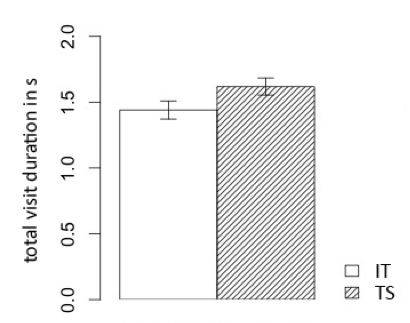
\includegraphics[height=.3\textheight]{figures/Fox6.png}
  \caption{Comparison of the average total visit duration of the IT und TS participants}
  \label{fox:fig:6}
\end{figure}


Another measurement of visual attention was defined as split-attention between image and title area. As the first hypothesis predicted shorter reading time, the second hypothesis predicted that the participants with integrated titles spend more time exploring the image than looking at the title. To test this hypothesis, TVD of both the entire image and the (sub)title area during the stimulus, meaning the time between the (sub)title fading in and out, was measured. For all four data sets (TVD of the image TS/IT and TVD of the title area TS/IT), the Shapiro-Wilk test showed a non-normally distributed population. The Wilcoxon test then showed highly significant differences between the corresponding data sets:


\ea
\begin{tabbing}
xxxxxxxxxxxxxxxxxxxxxxxxxxxxxxxxxxxxxxxx\=xxxxxxxssxxxxxxxxxxxx\kill
wilcox.test(TVD\_IT\_IMAGE, TVD\_IT\_TITLE): \>		W = 4400522, p < 0.001\\
wilcox.test(TVD\_TS\_IMAGE, TVD\_TS\_TITLE): \>		W = 2769346, p < 0.001\\
wilcox.test(TVD\_TS\_IMAGE, TVD\_IT\_IMAGE): \>		W = 2616334, p < 0.001\\
wilcox.test(TVD\_TS\_TITLE, TVD\_IT\_TITLE): \>		W = 2217703, p < 0.001
\end{tabbing}
\begin{tabbing}
xxxxxxxxxxxxxxxxxxxxxxxxxxxxxxxxx\=xxxxxxxxxxxxxxxxxxxxxxx\kill
m(TVD\_TS\_IMAGE) = 3.555 s	\>	m(TVD\_TS\_TITLE) = 1.835 s\\
m(TVD\_IT\_IMAGE) = 3.306 s	\>	m(TVD\_IT\_TITLE) = 1.570 s
\end{tabbing}
\z


The results show that on average the TS participants focused on the subtitle area for 51.6\% of the title display duration, on average 1.83s of 3.55s. For integrated titles, the participants focused on the title area for around 47.5\% of the time (on average 1.57s of 3.3s.; see Figure \ref{fox:fig:7}).


\begin{figure} 
  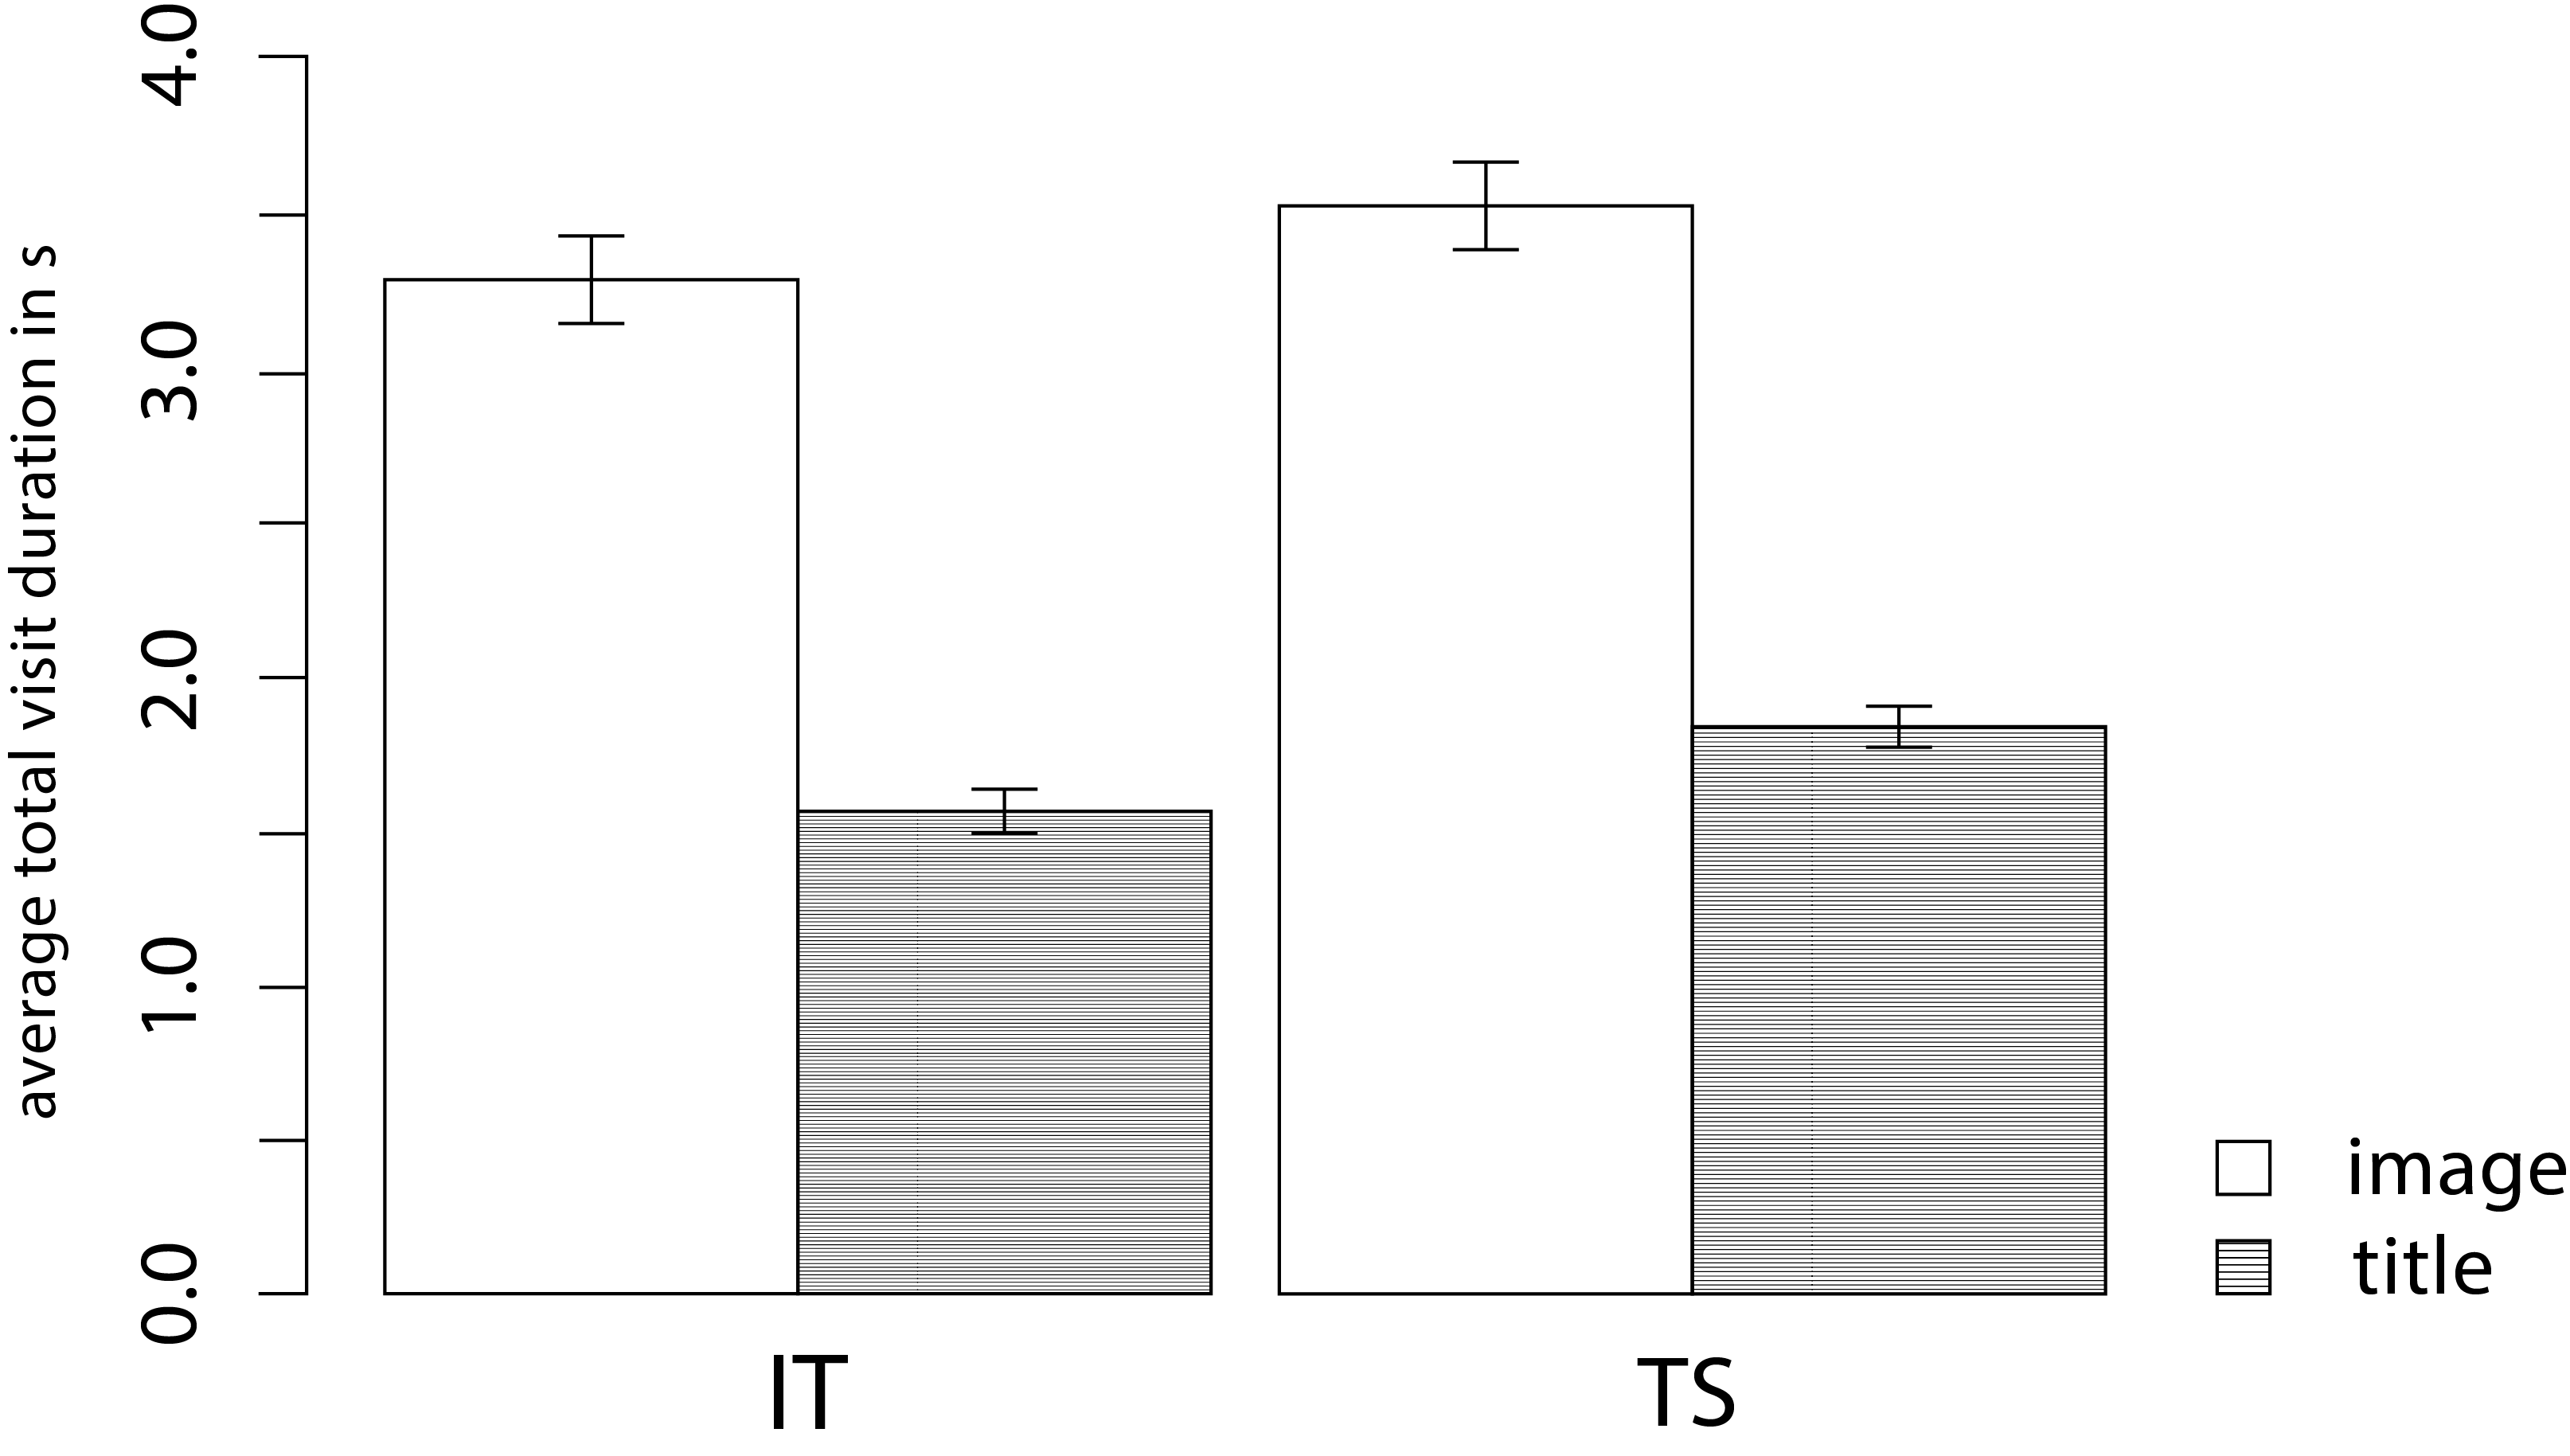
\includegraphics[height=.3\textheight]{figures/Fox7.png}
  \caption{Comparison of split-attention in IT and TS participants}
  \label{fox:fig:7}
\end{figure}

\begin{figure} 
  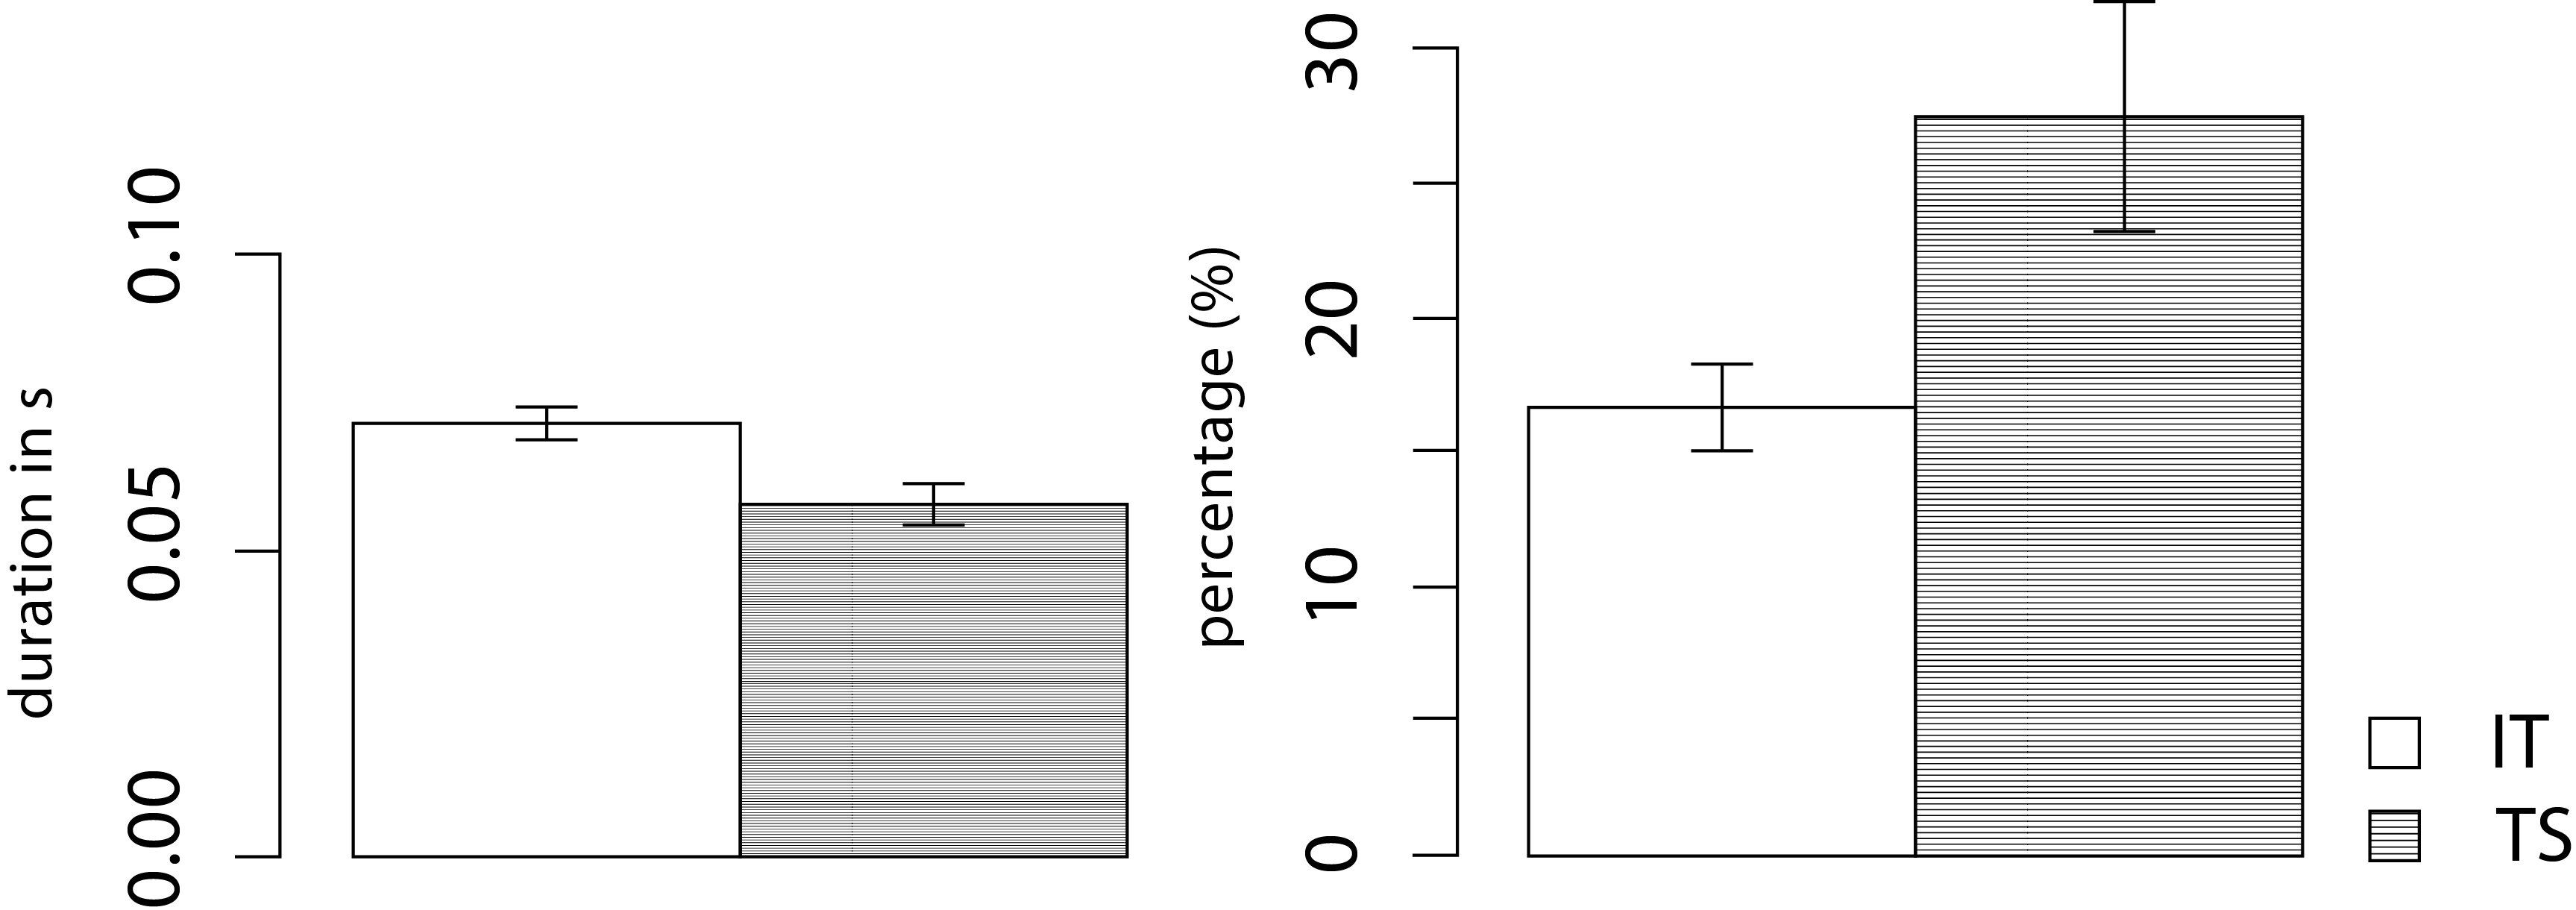
\includegraphics[height=.3\textheight]{figures/Fox8.png}
  \caption{Comparison of the average total visit duration of the IT und TS participants}
  \label{fox:fig:8}
\end{figure}


Due to the very short time frame in which the (sub)titles are visible, the difference seems quite small. Therefore, the explorative behaviour right before and after the stimulus should be examined. For the time frame right before the (sub)title is blended in, a look at the reaction times might be insightful. A reaction time of 0 means that a participant had already focused on the area before the (sub)title was shown. This value should only occur rarely, e.g. between sequential (sub)titles containing long sentences.



Figure \ref{fox:fig:8} shows the reaction times and corresponding average number of the value 0. For the IT participants, the value 0 occurred on average 23.1 times and 33.4 times for the TS participants; this corresponds to 16.5\% of all reaction times for the IT participants and about 27.5\% for the TS participants. Therefore, the TS participants focused on the title area before the stimulus significantly more often while the IT participants remained focused on the image for a longer time. An analysis of how long the audience’s gaze remained in the title area after the (sub)title had already faded out is planned for a follow-up study.



The third hypothesis stated that the IT participants are more likely to fixate the same focus points as the native participants. The hypothesis was tested using a random sample of corresponding subtitles and titles and automatically generated cluster areas. These clusters are areas with accumulated fixations and are generated by the Tobii Studio software (see \ref{fox:fig:9}).


\begin{figure} 
  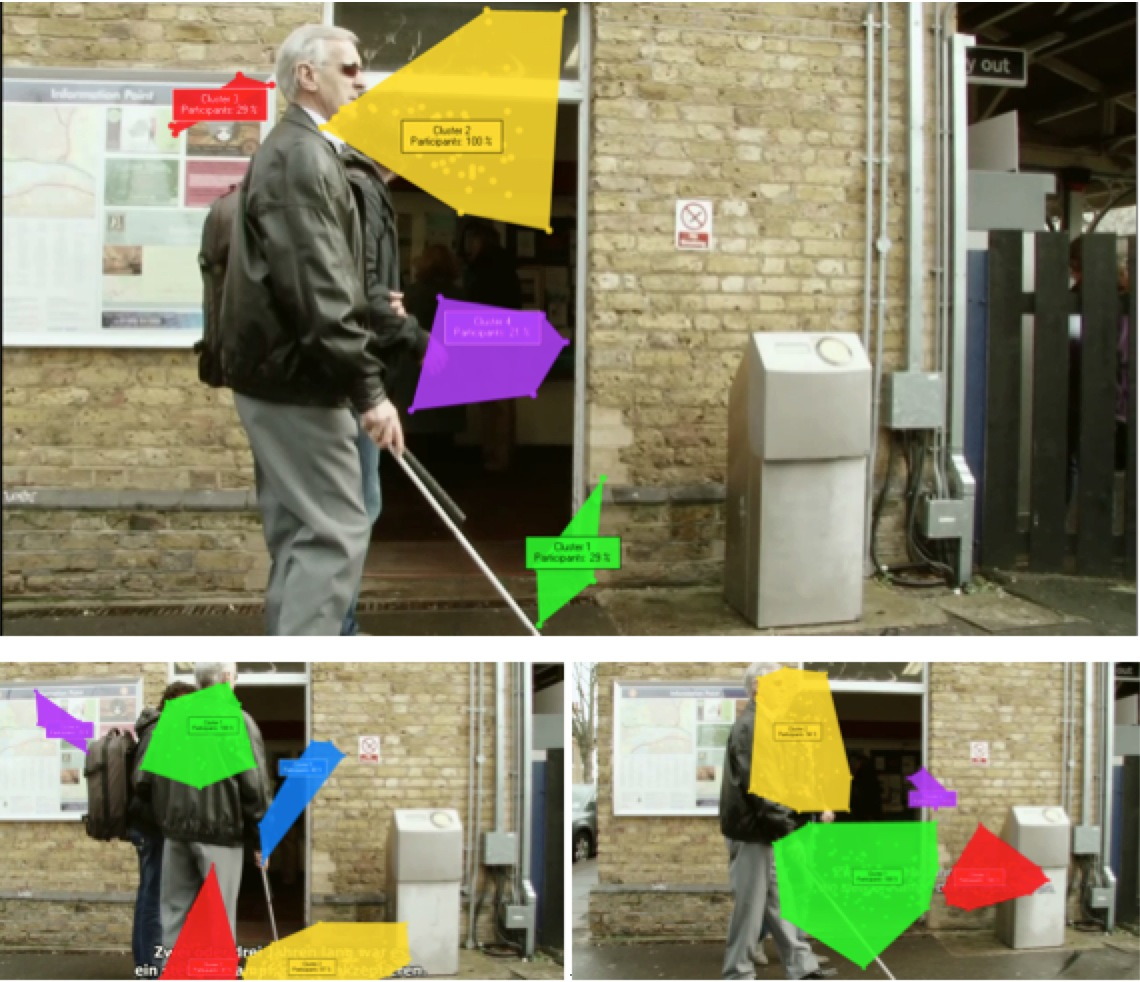
\includegraphics[height=.3\textheight]{figures/Fox9.png}
  \caption{Comparison of the automatically created clusters OV/TS/IT (Joining the Dots, UK 2012)}
  \label{fox:fig:9}
\end{figure}


These clusters were created for ten random scenes\footnote{Excluding scenes in which a subtitle (TS) was divided into several titles (IT) and scenes that consisted exclusively of a black background. The first few scenes only consisted of the film title and prologue and were therefore skipped. After that, every tenth scene was used. For detailed information, see Fox (in preparation).} and considered only when they were fixated by at least half of the corresponding participant group. Four clusters weren’t evaluated as they couldn’t be interpreted clearly while 23~clusters were evaluated. During this sample, the most relevant focus points – the clusters which at least 50\% of participants viewed – were fixated by an average 87.87\% of the OV~participants. Clusters at the same spot or very close were fixated by an average 75.3\% of the TS~participants and 83.3\% of the IT~participants. Thus, the integrated titles increased the mean number of participants that fixated the focus points of the English natives by 10.6\%. Additionally, the sample showed that, on average, 88.1\% of the TS participants fixated the subtitles while about 98.2\% of the IT participants fixated the integrated titles – an increase of 11.5\%. All in all, a higher percentage of the IT participants in this random sample focused both on the focus points of the OV participants and the displayed titles.



The hypothesis of increased reaction time due to integrated titles is based on the assumption that an audience that is used to subtitles has already learned to switch focus to the bottom area as soon as someone in the film starts speaking. For integrated titles, one can assume that the title area isn’t focused until the fade-in effect initiates the eye movement (cf. “involuntary attention”, Prinzmetal/McCool/Park 2005,~74). To test this hypothesis, areas of interest were defined for every subtitle and title. They allow measurements of the reaction time, meaning the duration between when the (sub)title fades in and the first fixation in the corresponding area of interest (“time to first fixation”, TFF). The data of the 15 TS and the 16 IT participants were compared and, as the Shapiro-Wilk test was significant for both data sets, the Wilcoxon test was applied: W = 2281026, p {\textless} 0.001. The reaction time of the IT participants (0.074s) was – taking the 0 values into account – on average 28.9\% higher (0.017s) than for the TS participants (0.057s). Omitting the 0 values, the increase was about 25.9\% – from 0.069s for TS participants to 0.087s for the IT participants; see Figure \ref{fox:fig:10}).



  
\begin{figure} 
  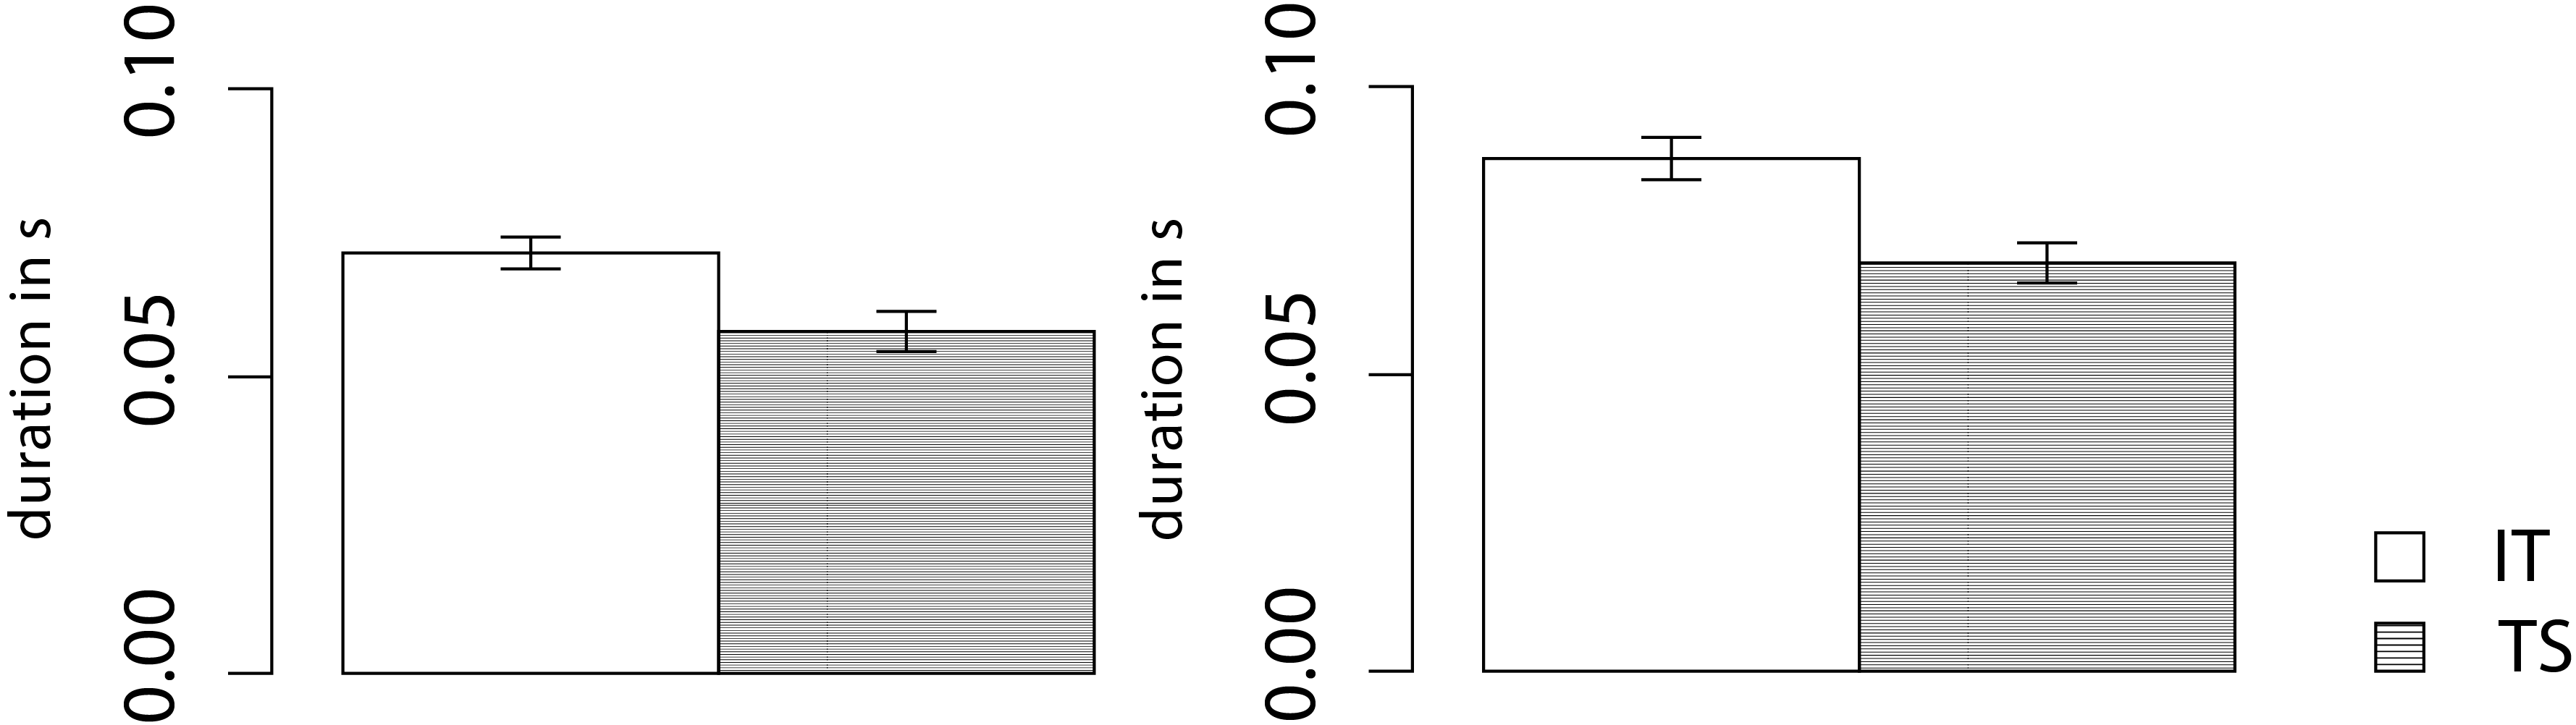
\includegraphics[height=.3\textheight]{figures/Fox10.png}
  \caption{Mean reaction time with (left) and without (right) the 0 values}
  \label{fox:fig:10}
\end{figure}
 

\subsection{Questionnaire results}

In addition to recording the eye movements and analysing the attention and reaction of the participants, a questionnaire on the aesthetic experience was also part of the study. As eye movements cannot tell us very much about the subjective feelings of a participant, all participants with integrated titles were asked to rank several statements after watching \textit{Joining the Dots}.\footnote{The questionnaire was designed following the recommendations on http://www.wpgs.de/content/blogcategory/87/355/ [06.01.2015].} The questionnaire was divided into a general part with statements on information intake and a second part focusing on the aesthetic experience. The participants could rank the statements on a four-point Likert scale from 1 (“I fully agree”) to 4 (“I completely disagree”). For a clearer presentation of the results, the first and second ranks were interpreted as “agreement” and the third and fourth rank as “disagreement”. All 16~participants with integrated titles rated all the statements anonymously. The following statements\footnote{It cannot be ruled out that a less positive wording of the statements would influence the overall agreement.} were to be ranked:

\begin{itemize}
\item I could easily read all integrated titles.
\item I received all necessary information through the integrated titles.
\item I would prefer integrated titles to traditional subtitles.
\item I could spend more time exploring the image compared to traditional titles.
\item Due to the integrated titles, I was aware of more details in the image.
\item The integrated titles didn’t cover important elements in the image.
\item The integrated titles distracted me less from the image compared to traditional subtitles.
\end{itemize}

\begin{figure}
 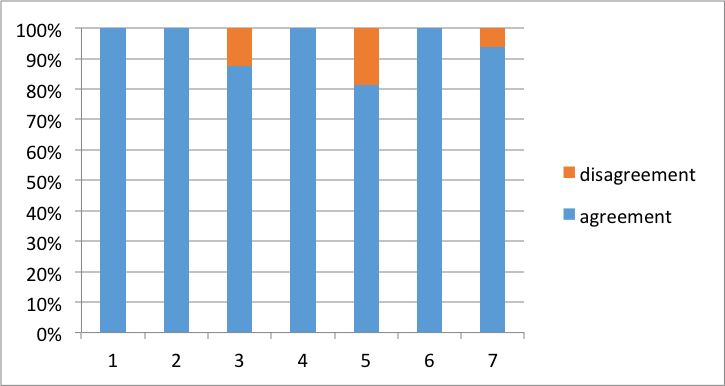
\includegraphics[width=\textwidth]{figures/Fox11.png}
 \caption{Distribution of agreement and disagreement with the statements}
 \label{fox:fig:11}
\end{figure} 




Figure \ref{fox:fig:11} shows that more than half of the participants agreed or fully agreed with the statements. While still scoring more than 80\% agreement, statement 5 on improved detail perception was agreed with least. In addition to the statements, the participants were asked to rate their aesthetic experience (“How would you rank your overall aesthetic experience with the integrated titles?”). Nine out of the 16 participants ranked it 1 (“very good”), 7 rated it 2 (“good”). None of the participants ranked it 3 (“satisfactory”) or 4 (“unsatisfactory”).


\section{Discussion}

This paper investigated whether integrated titles represent an advantageous alternative to traditional subtitles. The study used both eye tracking and questionnaire data to determine whether integrated titles offer improvements over traditional subtitles concerning visual attention, information absorption and aesthetic experience. In the first step, 14 native English-speaking participants watched the original version of the short documentary \textit{Joining the Dots}. This allowed a determination of the audience’s undistracted focus and yielded gaze data that could later be compared to the gaze data from participants reading (sub)titles. The analysis of the recorded focus points served as orientation for the best possible placement of the integrated titles. In the second step of the study, traditional German subtitles were added to the documentary and shown to 15 German speakers with little or no knowledge of English. This data could later be compared to the gaze behaviour of the third group, 16 native-speakers of German with little or no knowledge of English watching the documentary with integrated titles.


The average reading time for integrated titles decreased by about 14.4\% compared to the average reading time for traditional subtitles. While (sub)titles where visible, IT participants focused on the title area on average 47.5\% of the time and TS participants 51.6\%. This indicates that integrated titles motivate the audience to return to the actual focal point in the image faster and spend more time exploring the image while the title is visible. This is also supported by the low number of participants that fixated the title area before the title was faded in: Only about 16.5\% of all recorded reaction times of the IT participants was 0 (therefore they focused on the area before the recording time and display of the title; compare to “astray fixations” in Rajendran et al. 2012). For the TS participants, the percentage of reaction times amounting to 0 was 28.7\%. Therefore, about 1 out of 4 TS viewers wasted time they could have spent on the image by fixating the subtitle area too early (excluding successive subtitles that are part of the same sentence). A possible interpretation is that integrated titles trigger a more efficient reading, as both reading time and wasted time are reduced.



Looking at a random sample of ten (sub)titles and the therein defined 23~important areas of attention, the gaze behaviour of the TS and IT participants was compared to that of the 14~English native speakers. The automatically generated clusters, the areas of accumulated fixations created by Tobii Studio, were defined as relevant focus points if more than 50\% of the participants fixated them at least once. While on average 87.87\% of the OV participants fixated the 23 focus points, 75.3\% of the TS participants and 83.3\% of the IT participants fixated similar areas. In addition, an increase of 11.5\% of the participants that fixated the (sub)titles could be observed for the integrated titles: While on average 88,1\% of the subtitles were fixated by the TS participants, this number increased to 98.2\% for the integrated titles. This indicates that integrated titles allow for a more undistracted gaze behaviour and at the same time seem to motivate the viewer to fixate a higher percentage of the titles. It also invalidates the possible point of criticism that viewers might be more likely to miss a title due to the changing position.



The reaction time of the IT participants, however, increased visibly: Including the 0 values, the reaction time for integrated titles increased by 28.9\%, amounting to approximately 0.057s. Excluding the 0 values, the increase was about 25.9\% or 0.074s. An increased reaction time, however, cannot strictly be interpreted as a negative effect: While a shorter reaction time might be associated with less cognitive load for the viewer, a longer reaction time might also be synonymous with longer image exploration. Furthermore, the shorter reading time with a decrease of 0.265s on average seems to compensate the increased reaction time more than enough.



All in all, the evaluation of the eye tracking data shows that integrated titles can decrease the reading time and motivate the viewer to faster return to the relevant focus points. It seems less likely that the title area would be fixated before the title actually fades in and a random sample of ten scenes indicated that the focus of an audience using integrated titles is more likely to archive a similar gaze behaviour compared to the native participants. The reaction time increased.



The evaluation of the questionnaires resulted in an overall positive rating of their aesthetic experience by the German participants – especially when the integrated titles were compared to traditional subtitles. This positive feedback supports the hypothesis that differences in design and placement of (sub)titles are perceived by the audience and considerate placement can have positive impacts on the reception and information gain. Many participants that normally prefer dubbing, however, didn’t seem to see a possible alternative in the integrated titles. Participants used to traditional subtitles on the other side rated integrated titles as an improvement and a feasible alternative they would like to use in the future.



Practical implications arise for all areas of film translation. Film producers should be aware of the effects traditional subtitles can have on the film’s perception – especially in the light of top-grossing and award-winning Hollywood films making more profit in their translated versions than at home \citep[p. 202]{romero2013}. On the one hand, these rather basic eye tracking data already show the possible positive effect integrated titles can have on the information intake and aesthetic experience of the audience. On the other hand, a first set of basic modular guidelines for the creation of integrated titles were introduced in \citet{fox2015}. These offer new possibilities for filmmakers to have their work translated with more respect and to create a more aesthetic experience for the target audience.



As the integrated titles for \textit{Joining the Dots} were finalised after the third participant group watched the documentary using the eye tracker, a fourth study with 15 more German participants is planned to evaluate the possible impact of the adjusted text design and added effects. Additionally, the existing data set will be analysed with regard to the gaze behaviour directly after the title fades out. This will indicate whether the audience of integrated titles returns to the focal points in the image faster. The continuing work on integrated titles will include further development of the modular guidelines and the creation of comprehensible examples of placement and use of effects in various shot compositions without a graphic design or filmmaking background. The consideration and preservation of the typographic identity of film, e.g. the typefaces, colour sets and effects already used on text elements in the original version, is seen as a second relevant topic in the analysis of the graphical effects due to translation.\footnote{Presented in the talk “Reception, Information Flow and Aesthetics: Integrated Titles and Other Possible Improvements” during the \textit{International Conference on Eyetracking and Applied Linguistics 2014} in Warsaw and \textit{Languages \& The Media} \textit{2014} in Berlin.} Additionally, further studies might test the possibilities of integrated titles and accessibility-related adaptions – e.g. additional colour schemes for easier speaker identifications and the visualization of sound and noises. Such elements are already used in various contexts and can also be used to indicate the way someone speaks, their volume and intonation.



Overall, the study showed that integrated titles do have the potential to improve the viewing experience and offer film producers new angles of incorporating translation into their image compositions.


% \subsection*{References}
% 
% 
% Bannon, D. The Elements of Subtitles. A Practical Guide to the Art of Dialogue, Character, Context, Tone and Style in Subtitling. Lulu.com, 2009.
% 
% 
% 
% Döring, Sigrun. Kulturspezifika im Film: Probleme ihrer Translation. Berlin: Frank und Timme, 2006.
% 
% 
% 
% De Marco, Marcella. “Gender Portrayal in Dubbed and Subtitled Comedies.” Díaz Cintas, Jorge. New Trends in Audiovisual Translation. Multilingual Matters, 2009.
% 
% 
% 
% Delabastita, Dirk. “Translation and the Mass Media.” Bassnett, Susan and André Lefevere. Translation, History and Culture. London: Pinter Publishers, 1990. 97-109.
% 
% 
% 
% Díaz Cintas, Jorge and Gunilla Anderman. Audiovisual Translation. Palgrave Macmillan, 2009.
% 
% 
% 
% Díaz Cintas, Jorge. Media for All. Subtitling for the Deaf, Audio Description and Sign Language. Amsterdam: Rodopi, 2007.
% 
% 
% 
% —. New Trends in Audiovisual Translation. Bristol/Buffalo/Toronto: Multilingual Matters, 2009.
% 
% 
% 
% Dirscherl, Klaus. Bild und Text im Dialog. Passau: Wissenschaftsverlag Rothe, 1993.
% 
% 
% 
% Dries, Josephine. Guidelines for Production and Distribution. Düsseldorf: EIM, 1995.
% 
% 
% 
% “E-Teaching.” 2009. Eye Tracking. 21 Januar 2012 {\textless}http://www.e-teaching.org/didaktik/qualitaet/eye/{\textgreater}.
% 
% 
% 
% Fernández, María Jesús Fernández. “The Translation of Swearing in the Dubbing of the Film Southpark into Spanish.” Díaz Cintas, Jorge. New Trends in Audiovisual Translation. Multilingual Matters, 2009.
% 
% 
% 
% Flothow, Sebastian. “Hochschule RheinMain.” 24 Februar 2009. 26 Juni 2012 {\textless}http://www.cs.hs-rm.de/\~{}linn/fachsem0809/eyetracking/Eye\_Tracking.pdf{\textgreater}.
% 
% 
% 
% Göpferich, Susanne. Translationsprozessforschung: Stand, Methoden, Perspektiven. Tübingen: Narr, 2008.
% 
% 
% 
% Gambier, Yves. Multimedia Translation: Concepts, Practices and Research. Amsterdam: Bejamins, 2001.
% 
% 
% 
% Georgakopoulou, Panayota. “Subtitling for the DVD Industry.” Díaz Cintas, Jorge and Gunilla Anderman. Audiovisual Translation: Language Transfer on Screen. Palgrave Macmillan, 2009. 21-35.
% 
% 
% 
% Goldstein, Angelika. Foreign Language Movies - Dubbing vs. Subtitling: Lost in Translation or not? Hamburg: Kovac, 2009.
% 
% 
% 
% Hansen-Schirra, Silvia. “Multilingual Discourse Production: Diachronic and Synchronic Perspectives.” Kranich, Svenja, et al. Multilingual Discourse Production: Diachronic and Synchronic Perspectives. Amsterdam/Philadelphia: John Benjamins B.V., 2011. 135-162.
% 
% 
% 
% Ivarsson, Jan and Mary Carroll. Subtitling. Simrishamn: TransEdit, 2009.
% 
% 
% 
% Jüngst, Heike E. Audiovisuelles Übersetzen. Tübingen: Narr, 2010.
% 
% 
% 
% Joos, Markus, Matthias Rötting and Boris M. Velichkovsky. “TU Dresden.” 2002. 23 Mai 2012 {\textless}http://tu-dresden.de/die\_tu\_dresden/fakultaeten/fakultaet\_mathematik\_und\_naturwissenschaften/fachrichtung\_psychologie/i3/applied-cognition/publikationen/pdf/joos2002.pdf{\textgreater}.
% 
% 
% 
% Just, Marcel Adam and Patricia A. Carpenter. “A Theory of Reading: From Eye Fixations to Comprehension.” Psychological Review 1980: 329-354.
% 
% 
% 
% —. “Eye Fixations and Cognitive Processes.” Cognitive Psychology 1976: 441-480.
% 
% 
% 
% Kaakinen, Johanna K., Jukka Hyönä and Janice M. Keenan. “How Prior Knowledge, WMC, and Relevance of Information Affect Eye Fixations in Expository Text.” Journal of Experimental Psychology: Learning, Memory, and Cognition Vol. 29, No. 3 2003: 447-457.
% 
% 
% 
% Karamitroglou, Fotios. Towards a Methodology for the Investigation of Norms in Audiovisual Translation: The Choice between Subtitling and Revoicing in Greece. Amsterdam/Atlanta: Editions Rodopi B.V., 2000.
% 
% 
% 
% Ließner, S. Untertitelung einer Episode der BBC Sitcom {\textquotedbl}Yes Minister{\textquotedbl}. Essen: BDÜ, 1998.
% 
% 
% 
% Luyken, Georg-Michael. Overcoming Language Barriers in Television: Dubbing and Subtitling for the European Audience. Manchester: EIM, 1991.
% 
% 
% 
% Pettit, Zoë. “Connecting Cultures: Cultural Transfer in Subtitling and Dubbing.” Dìaz Cintas, Jorge. New Trends in Audiovisual Translation. Multilingual Matters, 2009.
% 
% 
% 
% “SEO Blog.” 2010. Eyetracking: Analyse des Nutzungsverhaltens. 11 April 2012 {\textless}http://www.myseosolution.de/eyetracking-analyse-webseite/{\textgreater}.
% 
% 
% 
% Traxler, Matthew J. and Martin J. Pickering. “Plausibility and the Processing of Unbounded Dependencies: An Eye-Tracking Study.” Journal of Memory and Language 35 1996: 454-475.
% %
% 
% %
% “UX Booth.” 2011. A Brief History of Eye-Tracking. 8 April 2012 {\textless}http://www.uxbooth.com/blog/a-brief-history-of-eye-tracking/{\textgreater}.
% 
% 
% 
% Vauras, Marja, Jukka Hyönä and Pekka Niemi. “Comprehending Coherent and Incoherent Texts: Evidence from Eye Movement Patterns and Recall Performance.” Journal of Research in Reading 15(1) 1992: 39-54.



\subsection*{Abbreviations}
\subsection*{Acknowledgements}


For their inexhaustible support and supervision, I would like to thank Prof. Dr. Silvia Hansen-Schirra, Dr. Pablo~Romero-Fresco and the MFG foundation in particular. Furthermore, special thanks go to Maik~Fox, Silke~Gutermuth, Rebecca~Klinkig, Jan Krämer, Dimitar~Molerov, Jean~Nitzke, Katharina Oster and Sascha~Wolfer for listening, discussing, reading and commenting on both small and larger scales.

\printbibliography[heading=subbibliography,notkeyword=this]

\end{document}

